\documentclass{article} 
\usepackage[utf8]{inputenc}
\usepackage{enumitem, amsmath, esint, systeme, graphicx, fontawesome5, titlesec}
\usepackage{MnSymbol}%
\usepackage{wasysym}%
% \usepackage[most]{tcolorbox}
\usepackage[scale=.95,type1]{cabin}
\usepackage[framemethod=tikz]{mdframed}
\graphicspath{ {./images/} }

\usepackage[legalpaper,margin=1in]{geometry}

\setlength{\parindent}{10pt}
% \setlength{\parskip}{1em}
\renewcommand{\baselinestretch}{1.2}

\title{Multiple Integrals}
\date{}
\author{}

\usepackage{tabularray}

\newcounter{Def}[section]
\newenvironment{Def}[1][]{%
  \ifstrempty{#1}%
  {\mdfsetup{%
    frametitle={%
      \tikz[baseline=(current bounding box.east),outer sep=0pt]
      \node[line width=1pt,anchor=east,rectangle,draw=blue!20,fill=white]
    {\strut \color{black}{Definition}~};}}
  }%
  {\mdfsetup{%
    frametitle={%
      \tikz[baseline=(current bounding box.east),outer sep=0pt]
      \node[line width=1pt,anchor=east,rectangle,draw=blue!20,fill=white]
    {\strut \color{black}{Definition}~:~\color{blue4}{#1}};}}%
  }%
  \mdfsetup{innertopmargin=2pt,linecolor=blue!20,%
            linewidth=1pt,topline=true,%
            frametitleaboveskip=\dimexpr-\ht\strutbox\relax,}
  \begin{mdframed}[]\relax%
  }{\end{mdframed}}

%%%%%%%%%%%%%%%% Integral
\makeatletter
%% make esint definition in line with amsmath
\@for\next:={int,iint,iiint,iiiint,dotsint,oint,oiint,sqint,sqiint,
  ointctrclockwise,ointclockwise,varointclockwise,varointctrclockwise,
  fint,varoiint,landupint,landdownint}\do{%
    \expandafter\edef\csname\next\endcsname{%
      \noexpand\DOTSI
      \expandafter\noexpand\csname\next op\endcsname
      \noexpand\ilimits@
    }%
  }
\makeatother


\mdfdefinestyle{theoremstyle}{%
linecolor=blue!20,middlelinewidth=1pt,%
frametitlerule=true,%
apptotikzsetting={\tikzset{mdfframetitlebackground/.append style={%
shade,left color=blue!20, right color=white}}},
frametitlerulecolor=white,
frametitlerulewidth=1pt,
innertopmargin=\topskip,
}
\mdtheorem[style=theoremstyle]{properties}{Properties}


\titleformat{\section}
  {\fontfamily{lmss}\selectfont\LARGE\bfseries\color{black}}
  {\thesection}{1em}{}
\begin{document}
\section{Double Integrals over Rectangles}
The Riemann sum 
\[\int_a^b f(x) \, dx = \lim_{n \to \inf } \sum_{i=1}^n f(x_i^{*}) \Delta x\]
\begin{center}
  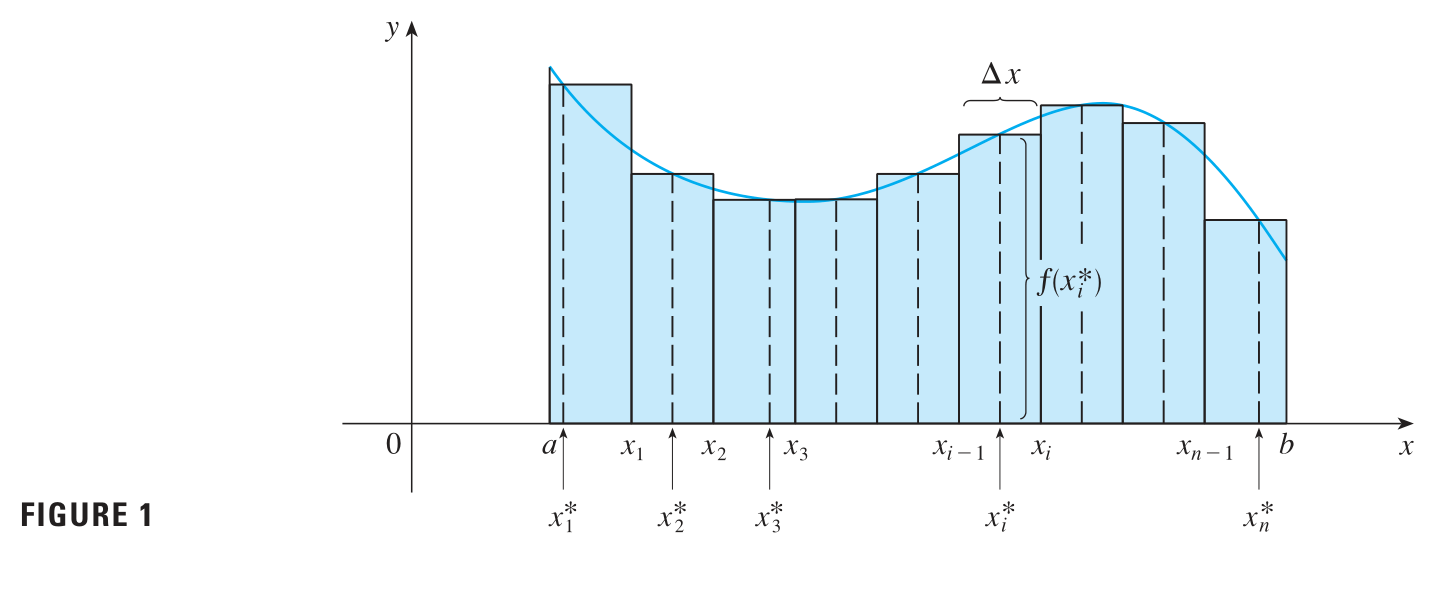
\includegraphics[width = 10 cm]{2dint.png} 
\end{center}
\subsection*{{\fontfamily{lmss}\selectfont \textcolor{blue5}{\faIcon{anchor} \underline{Volumes and Double Integrals}}}}

  Form the subrectangles 
  \[F_{ij} = [x _ {i - 1} , x _ y] \times [y _ {i - 1} , y _ i ] =  \{(x,y) \text{ } | \text{ } x _ {i - 1} \le x \le x_i, y _ {j-1} \le y \le y_j \} \]
each with area $\Delta A = \Delta x \Delta y$.
  \begin{center}
  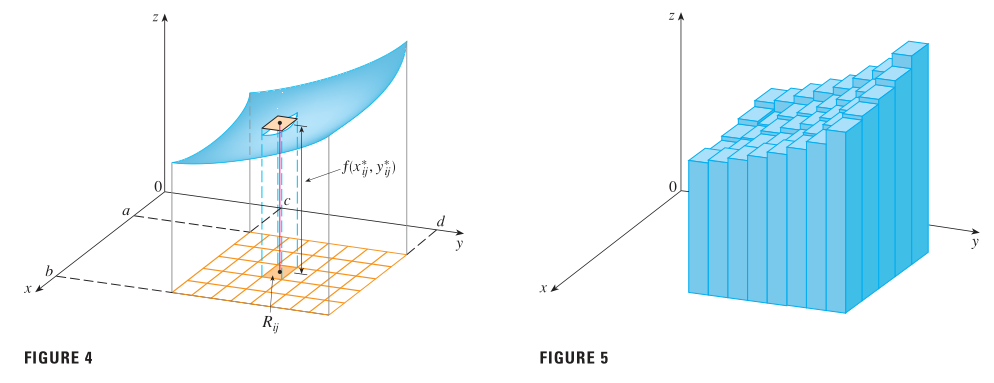
\includegraphics[width = 14 cm]{3dint_2} 
\end{center}
\begin{Def}[Double Integral]
  The \textbf{double integral} of $f$ over the rectangle $R $ is 
  \[ \iint \limits_{R} f(x,y) \, dA = V = \lim_{m, n \to \infty}\sum_{i=1}^m \sum_{j = 1}^n f(x _ {ij} ^* , y_{ij}^*) \Delta A\]
\end{Def}
{\fontfamily{lmtt}\selectfont \textbf{\textcolor{blue5}{\faIcon{map-marker-alt} EXAMPLE 1.}}} Estimate the volume 
\[R = [0,2] \times [0,2], \quad z = 16 - x^2 - 2 y^2 \]
Divide $R$ into 4 squares and choose the sample point to be the upper right corner of each square $R_{ij}$.
\begin{equation*}
  \begin{split}
    V & \approx \sum_{i = 1}^2 \sum_{j = 1}^2 f(x_i, y_j) \Delta A \\
    & = f(1,1) \Delta A  + f(1,2) \Delta A + f(2,1) \Delta A + f (2,2)\Delta A \\
    & = 13 (1) + 7 (1) + 10(1) + 4(1) = 34  
  \end{split}
\end{equation*}


\begin{minipage}[]{0.3\linewidth}
  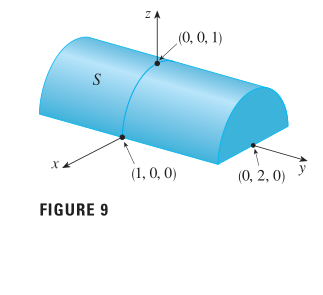
\includegraphics[width = 4.3 cm]{./images/cylinder.png}
  
\end{minipage}
\begin{minipage}[]{0.67\linewidth}
{\fontfamily{lmtt}\selectfont \textbf{\textcolor{blue5}{\faIcon{map-marker-alt} EXAMPLE.}}} If $R = \{(x,y) | -1 \le x \le 1, -2 \le y \le 2 \}$, evaluate 
\begin{equation*}
 \iint \limits_{R} \sqrt{1 - x^2 }\, dA 
\end{equation*}
Since $\sqrt{1 - x^2 } \ge 0 $, we can interpreting it as a volume. $x^2 + z^2 = 1$ and $z \ge 0$.
\[\iint \limits_{R} \sqrt{1 - x^2 }\, dA = \frac{1}{2} \pi (1)^2 \times 4 = 2 \pi\]
  
\end{minipage}

\subsection*{{\fontfamily{lmss}\selectfont \textcolor{blue5}{\faIcon{anchor} \underline{The Midpoint Rule}}}}
Take $(x_i*, y_i*) = (\overline{x_i}, \overline{y_i})$ (the middle point between $x_i, x_{i-1}$).

\begin{minipage}[]{0.3\linewidth}
 \begin{center}
   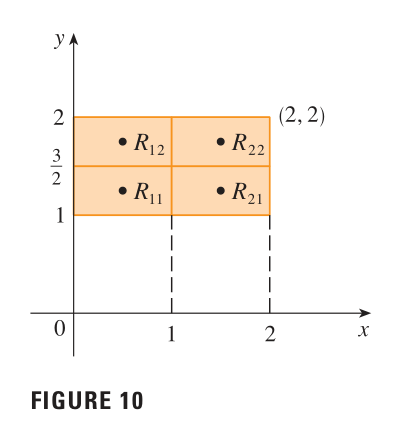
\includegraphics[width = 4.3 cm]{images/midpointruleeg1.png} 
 \end{center}
\end{minipage}
\begin{minipage}[]{0.67\linewidth}
{\fontfamily{lmtt}\selectfont \textbf{\textcolor{blue5}{\faIcon{map-marker-alt} EXAMPLE.}}} $m = n = 2$, $R = \{ (x, y) | 0 \le x \le 2, 1 \le y \le 2 \}$
\begin{equation*}
  \begin{split}
    \iint \limits_{R} (x - 3 y^2 )\,dA & \approx \sum_{i=1}^2 \sum_{j = 1}^2 f(\overline{x_i}, \overline{y_i}) \Delta A \\
                                       & = f(\overline{x_1}, \overline{y_1}) \Delta A  + \dots + f(\overline{x_2}, \overline{y_2}) \Delta A \\
                                       & = f(\frac{1}{2}, \frac{5 }{ 4 }) \Delta A + f(\frac{1 }{ 2 }, \frac{7 }{4 }) \Delta A     + f (\frac{3 }{ 2 } , \frac{5 }{ 4 } ) \Delta A + f ( \frac{3 }{ 2 } , \frac{7 }{4 }) \Delta A \\
                                       & = -11.875
  \end{split}
\end{equation*}
\end{minipage}\\
\textbf{\textcolor{blue5}{\fontfamily{lmss}\selectfont Note.}} Double integral as a bolume is valid only when $f$ is a \textit{positive} function. So in the previous example, the integral is not a volume.

\subsection*{{\fontfamily{lmss}\selectfont \textcolor{blue5}{\faIcon{anchor} \underline{Average Value}}}}
The average value of $f(x)$ on $(a,b)$ is $f_{ave} = \cfrac{1 }{b - a } \int_a^b f(x) \, dx $.
\begin{Def}[Average Value]
  The \textbf{average value} of $f(x,y)$ on a rectangle $R$ is 
  \[f_{\text{ave}} = \frac{1}{A(R)} \iint \limits_{R} f(x,y) \, dA\]
  If $f(x,y) \ge 0$, the equation $A(R) \times f_{\text{ave}} = \iint \limits_{R} f(x,y)\, dA$ says that it has the same $V$ as a box with base $R$ and height $f_{\text{ave}}$.
\end{Def} 
\subsection*{{\fontfamily{lmss}\selectfont \textcolor{blue5}{\faIcon{anchor} \underline{Properties of Double Integrals}}}}
The \textit{linearity} of the integral ($+, c\times$).

If $f(x,y) \ge g(x,y)$ for all $(x,y) \in R$, then  
\[\iint \limits_{R} f(x,y) \, dA \ge \iint \limits_{R} g(x,y) \, dA\]

\subsection*{{\fontfamily{lmss}\selectfont \textcolor{blue5}{\faIcon{anchor} \underline{Iterated Integrals}}}}
$\int_c^d f(x,y) \, dy$ means that $x$ is fixed and $f(x,y)$ is integrated with respecto $y$ from $c \to d$. (\textit{partial integration with respect to $y$}).

\begin{Def}[Iterated Integral]
  \[\int_c^d \int_a^b f(x,y) \,dx\,dy = \int_c^d \left[ \int_a^b f(x,y) \, dx \right] \, dy\]
  work from the inside out.
\end{Def}
{\fontfamily{lmtt}\selectfont \textbf{\textcolor{blue5}{\faIcon{map-marker-alt} EXAMPLE.}}} 
\begin{enumerate}[label = (\alph*)]
  \item  
    \begin{equation*}
      \begin{split}
        \int_0^3 \int_1^2 x^2 y \, dy \, dx & = \int_0^3 \left[ \int_1^2 x^2 y \, dy \right] \, dx \\ 
        & = \int_0^3 \cfrac{3 }{2 } x^2 \, dx = \cfrac{x^3 }{2 } = \cfrac{27 }{2 }
      \end{split}
    \end{equation*}
    
  \item 
    \begin{equation*}
      \begin{split}
        \int_1^2 \int_0^3 x^2y \, dx \, dy & = \int_1^2  \left[ \int_0^3 x^2y \, dx \right]\, dy \\
                                           & = \int_1^2 9y \, dy = 9 \cfrac{y^2}{2} \Bigg]_1^2 = \cfrac{27 }{ 2 }
      \end{split}
    \end{equation*}
    
     
\end{enumerate}

\begin{Def}[Fubini's Theorem]
  If $f$ is continuous on $R = \{ (x,y) \text{ } | \text{ } a \le x \le b , c \le y \le d  \}$, then 
  \[ \iint \limits_{R} f(x,y) \, dA = \int_a^b \int_c^d f(x,y) \,dy\,dx =  \int_c^d\int_a^b f(x,y) \,dx\,dy\]
\end{Def}

\begin{minipage}[]{0.3\linewidth}
  \begin{center}
    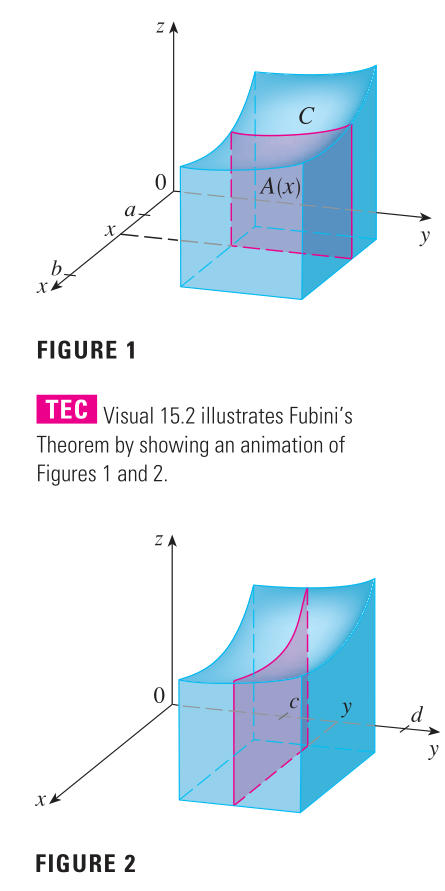
\includegraphics[width = 4.3 cm]{./images/fubini.png} 
  \end{center}
  
\end{minipage}
\begin{minipage}[]{0.67\linewidth}
  \[V = \int_a^b A(x)\,dx\]
  where $A(x)$ is the area of the surface that is perpendicular to the $x-$ axis.
  \[A(x) = \int_c^d f(x,y)\, dy\]


\end{minipage}  

\begin{Def}[Special case]
In case $f(x,y) = g(x) \, h(y)$,
\[\iint \limits_{R} g(x) h(y) \, dA = \int_a^b g(x)\, dx \int_c^d h(y)\, dy\]
  
\end{Def}
{\fontfamily{lmtt}\selectfont \textbf{\textcolor{blue5}{\faIcon{map-marker-alt} EXAMPLE.}}} $R = [0, \pi / 2 ] \times [0, \pi / 2   ]$, then 

\begin{equation*}
  \begin{split}
    \iint \limits_{R} \sin{x} \cos{y} \,dA& = \int_0^{\pi /2 } \sin{x} \int_0^{\pi /2}\cos{y} \,dy\\ 
                                          & = \left[ - \cos{x} \right]  _0^{\pi / 2 } \left[ \sin{y}  \right]_0^{\pi / 2  } = 1 \cdot 1 = 1
    \end{split}
\end{equation*}
\subsection*{{\fontfamily{lmss}\selectfont \textcolor{blue5}{\faIcon{anchor} \underline{Double Integrals over General Regions}}}}

\begin{minipage}[]{0.3\linewidth}
  \begin{center}
    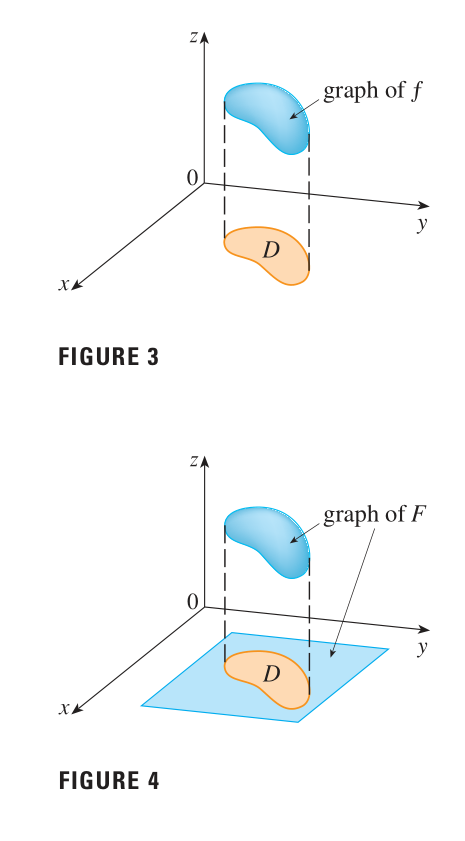
\includegraphics[width = 4.3 cm]{images/2intoverR.png} 
  \end{center}
  
\end{minipage}
\begin{minipage}[]{0.67\linewidth}
  The \textbf{double integral of $f$ over $D$}  is 
  \[\iint \limits_{D} f(x,y) \, dA = \iint \limits_{R} F(x,y)\,dA\]
  where $F(x,y) = \begin{cases}
    f(x,y) & \text{ if } (x,y) \text{ is in } D \\ 
    0 & \text{ if } (x,y) \text{ is in } R \text{ but not in } D 
  \end{cases}$    
\end{minipage}

\pagebreak
\subsubsection*{Type I: $D$ lies between 2 continuous function of $x$}
\[D = \{ (x,y) | a \le x \le b , g_1(x) \le y \le g_2(x) \}\]
   \begin{center}
     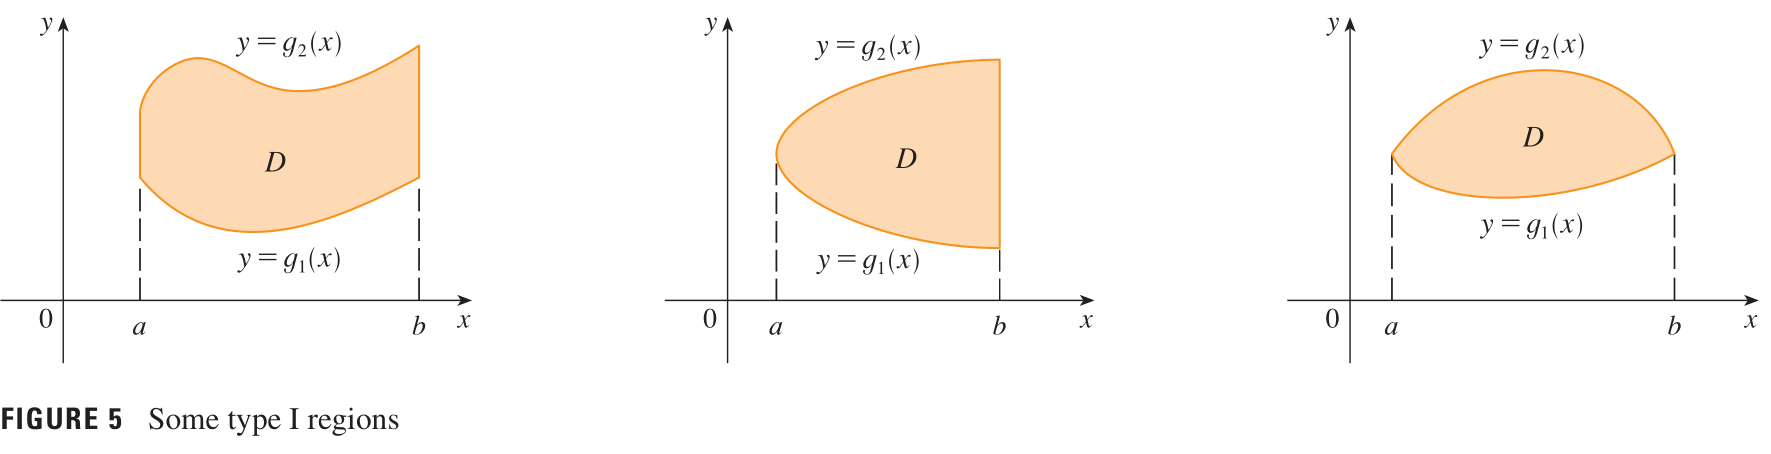
\includegraphics[width = 16 cm]{images/typeI.png} 
   \end{center}
\begin{Def}[Type I]
If $f$ is continuous on a type I region $D$ such that 
\[D = \{ (x,y) | a \le x \le b , g_1(x) \le y \le g_2(x) \}\]
then 
\[\iint \limits_{D} f(x,y) \, dA = \int_a^b \int_{g_1(x)}^{g_2(x)} f(x,y) \,dy\,dx\]
\end{Def}    
which leads to the definition for \textbf{Type II}, 
\[\iint \limits_{D} f(x,y) \,dA = \int_c^d \int_{h_1(y)}^{h_2(y)} f(x,y) \, dx \,dy\]

\begin{minipage}[]{0.3\linewidth}
  \begin{center}
    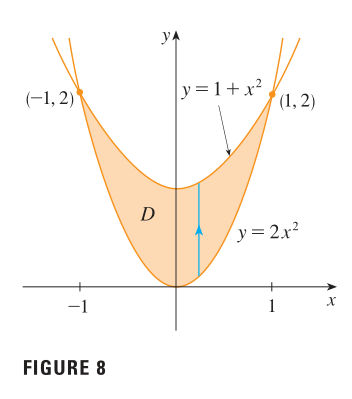
\includegraphics[width = 4.3 cm]{images/type1eg1.png} 
  \end{center}
  \end{minipage}
\begin{minipage}[]{0.67\linewidth}
{\fontfamily{lmtt}\selectfont \textbf{\textcolor{blue5}{\faIcon{map-marker-alt} EXAMPLE.}}} $y = 2x^2, y = 1 + x^2$, evaluate $\iint \limits_{D} (x + 2y) \, dA$.
\begin{equation*}
  \begin{split}
    \int \limits_{D } (x + 2y) \, dA & = \int_{-1}^1 \int_{2x^2}^{1+x^2} (x + 2y)  \, dy \, dx \\
                                     & = \int_{-1}^1 \left[ xy + y^2 \right]_{y - 2x^2}^{y = 1 + x^2}   \, dx \\
                                     & =  \int_{-1}^1 (-3x^4 - x^3 + 2x^2 + x + 1 ) \, dx \\ 
                                     & = \cfrac{32}{15} 
  \end{split}
\end{equation*}
\end{minipage}
 
\begin{minipage}[]{0.3\linewidth}
  \begin{center}
    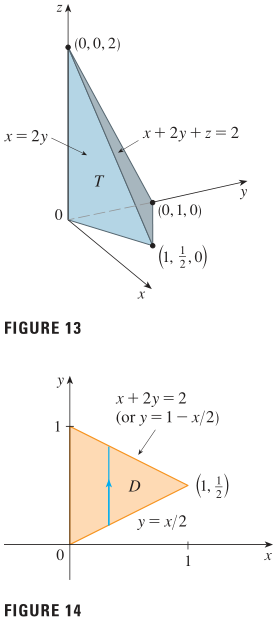
\includegraphics[width = 4.3 cm]{images/type2eg4.png} 
  \end{center}
  
\end{minipage}
\begin{minipage}[]{0.67\linewidth}
  {\fontfamily{lmtt}\selectfont \textbf{\textcolor{blue5}{\faIcon{map-marker-alt} EXAMPLE.}}} Find the volume of the tetrahedron bounded by the planes $x + 2y + z = 2, x = 2y. x = 0, z = 0 $.

  \[D = \big\{ (x,y) \text{ } | \text{ } 0 \le x \le 1, x/2 \le y \le 1 - x/2\big\}\]
  

\end{minipage}
\begin{minipage}[]{0.3\linewidth}
  \begin{center}
    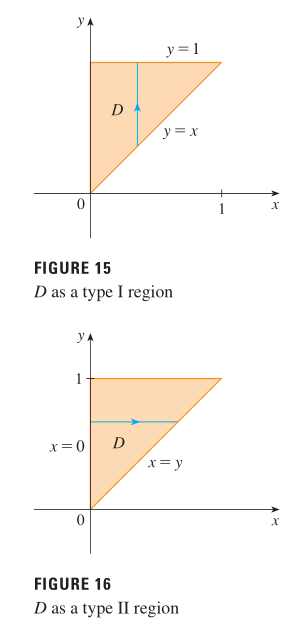
\includegraphics[width = 4.3 cm]{images/IIeg5.png} 
  \end{center}
  
\end{minipage}
\begin{minipage}[]{0.67\linewidth}
  {\fontfamily{lmtt}\selectfont \textbf{\textcolor{blue5}{\faIcon{map-marker-alt} EXAMPLE.}}} 
  \begin{equation*}
    \begin{split}
      \int_0^1 \int_x^1 \sin{(y^2)}\,dy\,dx & = \iint \limits_{D} \sin{(y^2)} \, dA  \\ D & = \big\{ (x,y) \text{ } | \text{ } 0 \le x \le 1, x \le y \le 1 \big\}
\end{split}   
  \end{equation*}
 can be transformed to 
 \[D = \big\{ (x,y) \text{ } | \text{ } 0 \le y \le 1, 0 \le x \le y \big\}\]
 
\begin{equation*}
  \begin{split}
    \int_0^1 \int_0^y \sin{(y^2)} \,dx \,dy &  = \int_0^1 \left[ x\sin{(y^2)} \right]  _{x=0}^{x = y} \, dy \\ 
                                            & = \int_0^1 y \sin{(y^2)} \, dy \\ 
                                            & = - \frac{1 }{2 } \cos{(y^2)} \big]_0^1 = \frac{1 }{2 } ( 1 - \cos{1  })
  \end{split}
\end{equation*}
\end{minipage}

\begin{properties}[Double Integrals]
  Beside sum and constant multiplier.

  \textcolor{blue5}{$\blacksquare$} If $f(x,y) \ge g(x,y)$ for all $(x,y) \in D $.
  \[\iint \limits_{D } f(x,y) \,dA \ge \iint \limits_{D } g(x,y) \, dA  \]

  
  \begin{minipage}[]{0.6 \linewidth}
  \textcolor{blue5}{$\blacksquare$} If $D = D_1 \cup D_2 $, and they don't overlap except perhaps on their bound daries 
  \[\iint \limits_{D}  f(x,y ) \, dA = \iint \limits_{D_1 } f(x,y) \, dA + \iint \limits_{D_2 }  f(x,y) \, dA \]
    
  \end{minipage}
  \begin{minipage}[]{0.3\linewidth}
    \begin{center}
      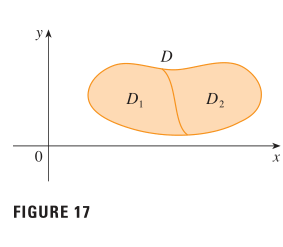
\includegraphics[width = 4.3  cm]{images/2domain.png} 
    \end{center}
  \end{minipage}
 
  \textcolor{blue5}{$\blacksquare$} Since $\iint \limits_{D }  1 \, dA = A(D )$, so if $m \le f(x,y) \le M $ for all $(x,y) \in D $.
  \[mA(D) \le \iint \limits_{D }  f(x,y ) \, DA \le MA(D )\]
\end{properties}

{\fontfamily{lmtt}\selectfont \textbf{\textcolor{blue5}{\faIcon{map-marker-alt} EXAMPLE.}}} Estimate $\iint \limits_{D }  e^{\sin{x} \cos{y}} \, dA $, where $D $ is the disk with center the origin and $r = 2 $. 

Since $-1 \le \sin{x} \le 1 $ and $-1 \le \cos{y} \le 1 $, we have $-1 \le \sin{x}\cos{y} \le 1 $. Therefore 
\[e^{-1} \le e^{\sin{x}\cos{y}} \le e^1  \]
\[\frac{4\pi }{e }  \le \iint \limits_{D }  e^{\sin{x} \cos{y}} \, dA \le 4 \pi e \]


\section{Double Integrals in Polar Coordinate}

\begin{minipage}[]{0.55\linewidth}
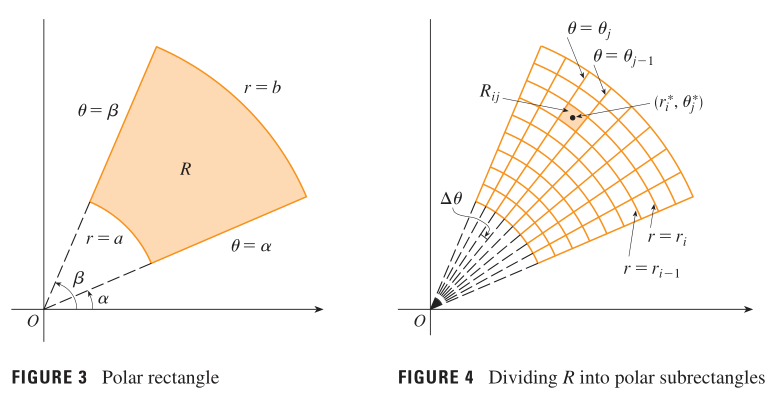
\includegraphics[width = 9 cm]{./images/explainpolar.png}
\end{minipage}
\begin{minipage}[]{0.42\linewidth}
    Divide into $m$ subinterval $[r_{i-1}, r_i]$ of $\Delta r = (b - a)/m$ and $n$ subinterval of $(\beta - \alpha)/ n $.

  \textcolor{blue5}{\small $\blacksquare$} Then the center of the polar subrectangles has polar coordinate \[r_i* = \frac{1 }{2 } (r_{i-1} + r_i ), \quad \theta_j* = \frac{1 }{2 } (\theta _ {j-1} + \theta_j)\]

   \textcolor{blue5}{\small $\blacksquare$} And the area 
   \begin{equation*}
     \begin{split}
       \Delta A_i & = \frac{1}{2} (r_i + r_{i-1})(r_i - r_{i-1})\Delta \theta \\ 
       & = r_i^* \Delta r \Delta \theta
     \end{split}
   \end{equation*}
   
\end{minipage}

\begin{Def}[Change to Polar Coordinates in a Double Integral]
  If $f$ is continuous on a polar rectangle $R$ ($0 \le a \le r \le b, \alpha \le \theta \le \beta$, where $0 \le \beta - \alpha  \le 2 \pi$), then 
  
  \begin{minipage}[]{0.25\linewidth}
    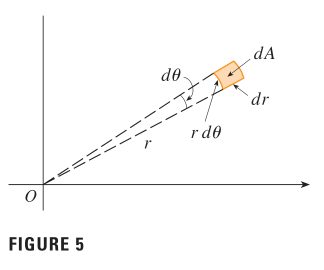
\includegraphics[width = 3.8 cm]{./images/polarimg.png}
    
  \end{minipage}
  \begin{minipage}[]{0.57\linewidth}
  \[\iint \limits_{R}  f(x,y) \ dA = \int_\alpha^\beta \int_a^b f(r \cos{\theta}, r \sin{\theta}) \, r \, dr \, d \theta\]
    \end{minipage}

    \begin{minipage}[]{0.25\linewidth}  
      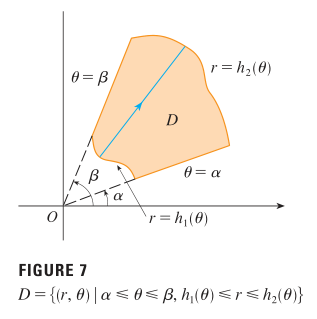
\includegraphics[width = 3.8 cm]{./images/polarimg2.png}
          
    \end{minipage}
    \begin{minipage}[]{0.57\linewidth}
      \[\iint \limits_{D} f(x,y)\, dA = \int_\alpha^\beta \int_{h_1(\theta)}^{h_2(\theta)} f(r \cos{\theta}, r \sin{\theta}) r \, dr \, d\theta\]
    \end{minipage}
\end{Def}

{\fontfamily{lmtt}\selectfont \textbf{\textcolor{blue5}{\faIcon{map-marker-alt} EXAMPLE.}}} Find the area enclosed by one loop of the four-leaved rose $r = \cos{2\theta}$.

\begin{minipage}[]{0.3\linewidth}
  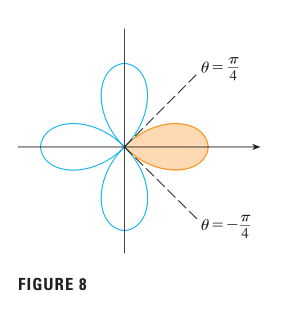
\includegraphics[width=4.3 cm]{images/2022-04-03-18-29-01.png}
\end{minipage}
\begin{minipage}[]{0.67\linewidth}
  \[D = \{(r, \theta) \text{ }  | \text{ } -\pi/4 \le \theta \le \pi/4, 0 \le r \le \cos{2\theta }\}\]
  So the area is 
    \begin{equation*}
        \begin{split}
            A(D) & = \iint \limits_{D }\, dA = \int_{- \pi / 4 }^{\pi / 4   } \int_0^{\cos{2\theta}} r \,dr\,d\theta \\ 
                 & =\int_{- \pi / 4 }^{\pi / 4   }  \left[ \frac{1}{2}r^2  \right]_0^{\cos{2\theta}} = \frac{1}{2}\int_{- \pi / 4 }^{\pi / 4   }  \cos{2\theta}^2 \, d\theta \\ 
                 & = \frac{1}{4} \int_{- \pi / 4 }^{\pi / 4   } ( 1 + \cos{4 \theta }) \, d\theta = \frac{1}{4}  \left[ \theta + \frac{1}{4} \sin{4 \theta } \right]_{- \pi /4 }^{\pi / 4    } = \frac{\pi }{ 8 }
        \end{split}
    \end{equation*}
    
  \end{minipage}
 
  {\fontfamily{lmtt}\selectfont \textbf{\textcolor{blue5}{\faIcon{map-marker-alt} EXAMPLE.}}}  $z = x^2 + y^2 $, $x^2 + y^2 = 2x $.

  \begin{center}
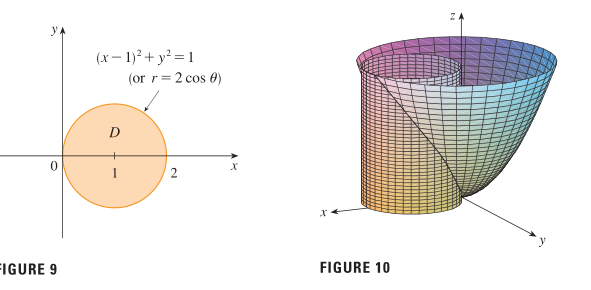
\includegraphics[width=10 cm]{images/2022-04-04-14-21-24.png}
    \end{center}  


% x = rcosx + 1, y = r sin x 
\[D = \{ (r, \theta) \text{ } | \text{ } -\pi / 2 \le \theta \le \pi / 2 , 0 \le r \le 2 \cos{\theta } \} \]
\begin{equation*}
  \begin{split}
    V & \iint \limits_{D } (x^2 + y ^2 ) \, dA =  \int_{ -\pi /2 }^{\pi /2  } \int_{0}^{2 \cos{theta }} r^2 r \, dr \, d \theta \\ 
      & = 4 \int_{-\pi / 2  }^{\pi / 2  } \cos{\theta}^4 \, d\theta = 8 \int_0^{\pi / 2 } \cos{\theta}^4 \, d\theta = 8 \int_0^{\pi / 2} \left( \frac{1 + \cos{2\theta}}{2 } \right)^2 \, d\theta \\ 
      & = 2 \left[ \frac{3}{2} \theta + \sin{2\theta}  + \frac{1}{8} \sin{4\theta}\right]_0^{\pi / 2  } = 2 \left( \cfrac{3 }{2 }  \right) \left( \cfrac{\pi }{2 } \right) = \cfrac{3 \pi }{2 } 
  \end{split}
\end{equation*}
Why split into 2 parts?



\end{document}
